\section{Algoritmi di Scheduling}

\subsection{Selezione}
Prima di vendere alcuni degli algoritmi più utilizzati dai sistemi operativi moderni vediamo il metodo che viene utilizzato per confrontare e migliorare gli algoritmi.

\subsubsection{Modelli Deterministici}
Nella valutazione analitica, si seleziona un set predeterminato di processi, e si simulano più algoritmi calcolandone il tempo medio di attesa nei vari casi.

\spacer
È possibile utilizzare la \textbf{Formula di Little} per avvicinarsi di più alla realtà:
Sia $n$ la lunghezza media della coda, $W$ il tempo medio di attesa e $\lambda$ il numero di processi in arrivo per unità di tempo. Allora $n = W \cdot \lambda$.

\subsubsection{Simulazione}
La simulazione implica la creazione di un modello del sistema di calcolo e un processo di logging dei dati.

\subsection{Algoritmi Comuni}

\subsubsection{First Come First Serve}
Un semplice algoritmo che fornisce le risorse al primo processo che le richiedono. Il criterio poi segue l'implementazione della coda FIFO, quando le risorse si liberano vengono assegnate al primo processo della coda.

Questa strategia non è efficace per i computer consumer in quanto un processo molto lungo può fermare l'esecuzione di altri processi brevi che l'utente richiede con maggiore urgenza.

\subsubsection{Highest Priority/Shortest Job First}
Viene fornito un valore di priorità ad ogni processo, le risorse vengono assegnate al processo con la priorità più alta.

Questo algoritmo presenta spesso il problema della \textit{starvation} dove i processi a priorità bassa non vengono mai eseguiti, ma introducendo l'\textit{aging} la priorità di un processo aumenta all'aumentare del suo tempo di attesa.

\subsubsection{Round Robin o Scheduling Circolare}
A ciascun processo vengono assegnate le risorse per un periodo di tempo limitato, solitamente 10-100 ms (un periodo più breve ha troppo overhead di switching, con uno più grande si ottiene un algoritmo FIFO)

Questo algoritmo ha in media un tempo medio di attesa maggiore di un algoritmo basato sulla priorità, ma ha un miglior tempo di risposta, cosa importante nei sistemi consumer.

\begin{figure}[H]
    \centering
    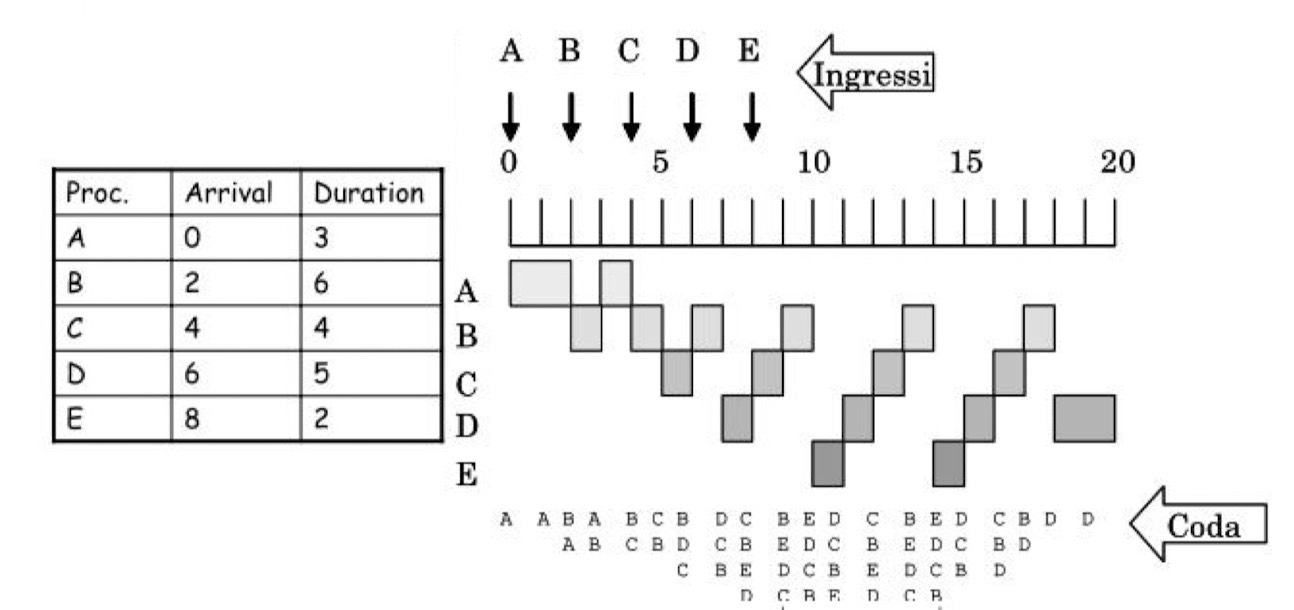
\includegraphics[width=0.65\linewidth]{assets/round-robin.jpg}
    \caption{Esempio di esecuzione dell'algoritmo}
\end{figure}

\begin{note}
    Spesso negli esercizi capita che un nuovo processo venga inserito nella coda ready allo stesso momento in cui un processo termina il suo quanto di tempo. Si incorre quindi in una situazione dove non è chiaro quale dei due processi verrà inserito prima nella ready queue.

    In questo caso è possibile scegliere la soluzione che si preferisce, con l'unico limite di restare consistenti all'interno dell'esercizio.
\end{note}

\subsubsection{Highest Response Ratio}
Definiamo un valore da utilizzare come priorità, la priorità del processo $P_i$ sarà $p_i = \frac{a_i + e_i}{e_i}$

Dove $a_i$ è il tempo di attesa del processo nello stato ready e $e_i$ è il tempo di esecuzione stimato.

\spacer
Questo significa che i processi brevi avranno una priorità maggiore, ma implementa anche l'\textit{aging} per evitare la \textit{starvation}.

\subsubsection{Code Multiple}
Come spesso accade la migliore soluzione vede l'utilizzo di più algoritmi allo stesso tempo, è possibile infatti costruire più code, tutte con algoritmi di gestione diversi. Poi sarà sufficiente allocare una certa percentuale di risorse ad ognuna delle code.

\subsubsection{Esempio 1.}
Questa strategia si può ad esempio utilizzare per dividere i processi che eseguono in foregorund e quelli in background. La coda in foreground avrà maggiore disponibilità di risorse e sarà gestita in Round Robin per assicurarsi un ottima esperienza utente, quella background avrà meno risorse a disposizione e sarà gestita in FIFO.

\subsubsection{Esempio 2.}
Le code multiple si possono utilizzare anche per implementare l'aging, ad esempio possiamo implementare 3 code nel seguente modo:

La prima e la seconda in Round Robin a 8 ms ed a 16 ms e l'ultima in FIFO.
In questo modo i processi ricevono tutti rapidamente 8 e poi 16 ms di tempo di esecuzione, risolvendo così i processi semplici, mentre i processi più lunghi finiscono nella coda FIFO e verranno eseguiti quando possibile.

\begin{figure}[H]
    \centering
    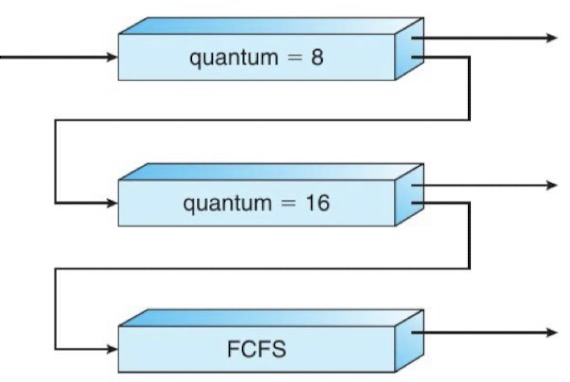
\includegraphics[width=0.32\linewidth]{assets/code-multiple.jpg}
\end{figure}

\subsubsection{Scheduling con Priorità Proporzionale alla frequenza}
Un caso tipico industriale è quello in cui i processi devono essere eseguiti ad intervalli regolari. In questo caso è conveniente definire una priorità proporzionale alla frequenza. Quindi processi che utilizzano la CPU con più frequenza avranno priorità maggiore.

\spacer
Questo è un algoritmo ottimale, quindi se esso non riesce a pianificare l'esecuzione di una serie di processi rispettando i vincoli temporali allora nessun altro algoritmo ci riuscirà.
\begin{figure}[H]
    \centering
    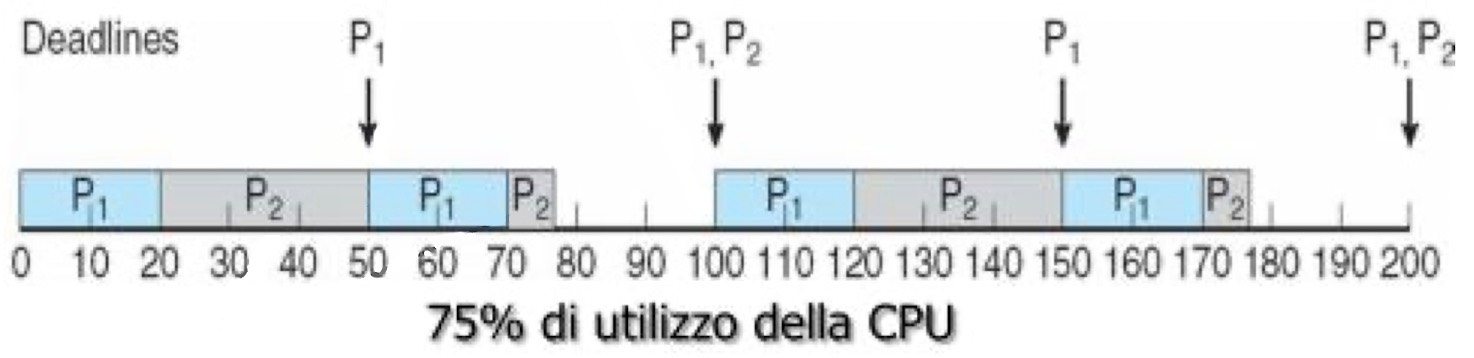
\includegraphics[width=0.6\linewidth]{assets/coda-frequenza.jpg}
\end{figure}

È possibile calcolare a priori se i processi potranno essere eseguiti rispettando i vincoli tramite la seguente formula:
$$\sum_{i=1}^{m}\frac{C_i}{P_i} \le m\cdot(2^{\frac{1}{m}} - 1)$$
dove m è il numero di processi $P_i$ il periodo del processo $i$ e $C_i$ la sua durata.

\subsubsection{Earliest Deadline First}
Assegna le priorità dinamicamente a seconda delle scadenze. Ogni processo per poter essere eseguito deve annunciare la sua prossima scadenza allo scheduler, più questa scadenza si avvicina più la priorità del processo aumenta.

\subsubsection{Esempio}
Siano due processi $P_1$ e $P_2$ con periodo di 50 e 80 e con tempo di esecuzione di 25 e 35.
\begin{figure}[H]
    \centering
    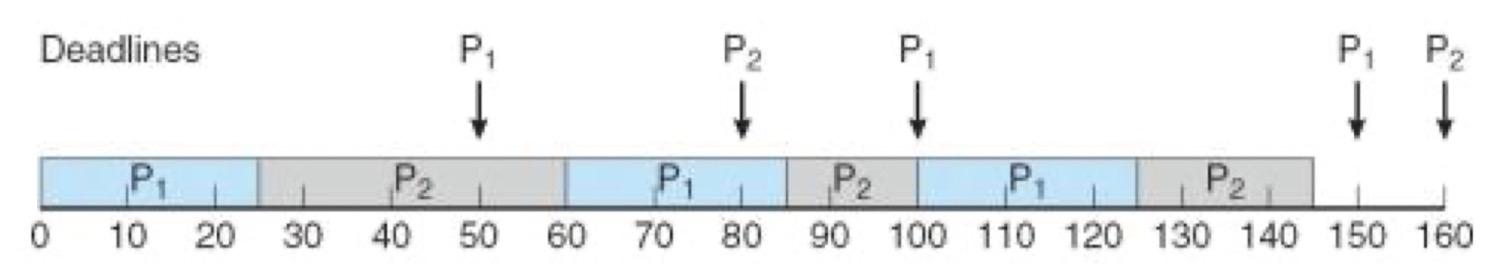
\includegraphics[width=0.6\linewidth]{assets/edf.jpg}
\end{figure}
Dalla figura si può vedere come a t=100 il processo $P_1$ interrompe $P_2$ in quanto la sua deadline è a t=150 mentre $P_2$ ha come deadline t=160
